%Used template from: https://github.com/jpeisenbarth/SRS-Tex
\documentclass{scrreprt}
\usepackage{listings}
\usepackage{underscore}
\usepackage[bookmarks=true]{hyperref}
\usepackage[utf8]{inputenc}
\usepackage[english]{babel}
\usepackage{graphicx}
\usepackage{xcolor}
\graphicspath{ {./images/} }
\hypersetup{
    bookmarks=false,    % show bookmarks bar?
    pdftitle={Software Design Specifications},    % title
    pdfauthor={Saad Ismail, Shehryar Naeem, Hassan Berry},                     % author
    pdfsubject={TeX and LaTeX},                        % subject of the document
    pdfkeywords={TeX, LaTeX, graphics, images}, % list of keywords
    colorlinks=true,       % false: boxed links; true: colored links
    linkcolor=blue,       % color of internal links
    citecolor=black,       % color of links to bibliography
    filecolor=black,        % color of file links
    urlcolor=purple,        % color of external links
    linktoc=page            % only page is linked
}%
\def\myversion{1.0 }
\date{}
%\title
\usepackage{hyperref}
\begin{document}

\begin{flushright}
    \rule{16cm}{5pt}\vskip1cm
    \begin{bfseries}
        \Huge{SOFTWARE DESIGN\\ SPECIFICATIONS}\\
        \vspace{1.9cm}
        for\\
        \vspace{1.9cm}
        Crowd Fund Raising\\
        \vspace{1.9cm}
        Prepared by\\Hassan Berry, Shehryar Naeem, Saad Ismail\\
        \vspace{1.9cm}
        FAST-NUCES Karachi\\
        \vspace{1.9cm}
        December 3, 2018\\
    \end{bfseries}
\end{flushright}

\chapter*{Document History}

\begin{center}
    \begin{tabular}{|c|c|c|c|}
        \hline
	    Version & Name of Person & Date & Description of Change\\
        \hline
	    1 & Hassan Berry & 01-12-2018 & Document Created\\
        \hline
        2 & Hassan Berry & 04-12-2018 & Document Completed\\
        \hline
        3 & Saad Ismail & 06-12-2018 & Document Converted to LaTeX\\
        \hline
        4 & Saad Ismail & 06-12-2018 & Proof-read\\
        \hline
        
    \end{tabular}
\end{center}

\chapter*{Distribution List}

\begin{center}
    \begin{tabular}{|c|c|}
        \hline
	    Name & Role\\
        \hline
	    Ms. Rubab Jaffar & Supervisor\\
        \hline
	    Mr. Awais Ahmed & Co-Supervisor\\
        \hline
    \end{tabular}
\end{center}

\chapter*{Document Information}

\begin{center}
    \begin{tabular}{|c|c|}
        \hline
	    Category & Information\\
        \hline
        Customer & FAST-NU Karachi\\
        \hline
        Project & Crowd Fund Raising\\
        \hline
        Document & Software Design Specification\\
        \hline
        Document Version & 1.0\\
        \hline
        Status & Final\\
        \hline
        Author(s) & Hassan Berry, Saad Ismail, Shehryar Naeem\\
        \hline
        Approver(s) &\\
        \hline
        Distribution & Supervisor,Co-Supervisor\\
        \hline
        
    \end{tabular}
\end{center}

\tableofcontents

\chapter{Introduction}

\section{Purpose of Document}
This document provides explicit information about the requirements of our project and how the project is put together. This document also documents the design methodology that we will be using for the project.

\section{Intended Audience}
Any engineers who might  get the job of improving our system to add further functionalities and will need to understand how the system was designed in the first place. Additionally; our supervisors who will grade us based on how correct, concise, and complete this document is.

\section{Document Convention}
Latex document class: scrreprt

\section{Project Overview}
The project is a web application which allows users of different types to interact with the Interface and get their specific requirements fulfilled. The purpose of the software is to allow companies, startups and individuals to interact on a common platform and exchange monetary benefits via sponsoring an idea, or donation to a cause. 

\section{Scope}
This project will consist of creating a marketable, and deployable application based on the concept of crowdsourcing and crowdfunding. The modules of the project will in include a mobile application and web based front end where users can interact with the database.
\subsection{Deliverables}
\begin{itemize}
  \item Functional Database
  \item Web based application
\end{itemize}

\chapter{Design Considerations}
The following design considerations need to be kept in mind:

\begin{enumerate}
  \item The User needs to access a website which is both visually appealing, and fast. All other functionalities come later.
  \item The database needs to handle multiple users at one time.
  \item All the functionalities must be present, in addition to the new features which will make loyal users.
\end{enumerate}

\section{Assumptions and Dependencies}
Assumptions:
\begin{itemize}
  \item The Users like a floating banner.
  \item The Users like dynamic websites.
  \item The User like categories to show up at the top.
\end{itemize}

\chapter{System Architecture}

\section{System Level Architecture}
Elements:
\begin{itemize}
  \item User
  \item Administrator
  \item Database
  \item User Interface
\end{itemize}

Relationships:
\begin{itemize}
    \item User interacts with User Interface to login, register, add category, post projects etc.
    \item Administrator interacts with Database to add new categories and check registered users.
\end{itemize}

User Interface Requirements:
\begin{itemize}
    \item The User Interface needs to be designed in a way that is functionally capable, visually attractive and is mobile-responsive.
\end{itemize}
\newpage

\subsection{Software Architecture}
We are using 3-tier architecture. The user only interacts with the front-end application (Angular 2) which requests back-end application (Node.JS) which then further fetches the data from the database (MySQL).

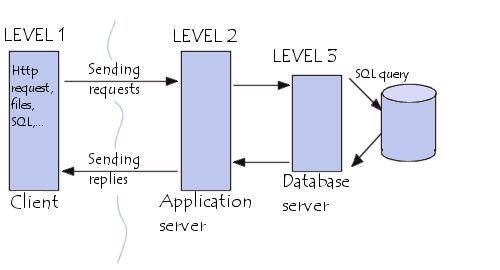
\includegraphics[width=\textwidth]{3tier.jpeg}
\newpage

\section{Design Strategy}
Our design strategy is focused on two main aspects:
\begin{itemize}
    \item Ease of Use
    \item Aesthetics
\end{itemize}

We believe that a website that is aesthetically pleasing to look at and  easy to navigate will definitely pull customers in and increase traffic, which is the prime goal of creating any website.

The next goal is to be functionally reliable, and we will ensure that happens so that we can build a web base of loyal customers.

\subsection{Future system extension}
\begin{enumerate}
    \item We will develop a mobile application on Android and iOS.
    \item We will add further functionalities to our current system like crowd-sourcing.
    \item We will 
\end{enumerate}

\subsection{System Reuse}
Our system is designed in a way that it can be reused again and again on different hosting services and can be connected to different databases.

\subsection{Data Management}
This part of our project is still ongoing.

\section{Detailed System Design}
\subsection{Database Design}
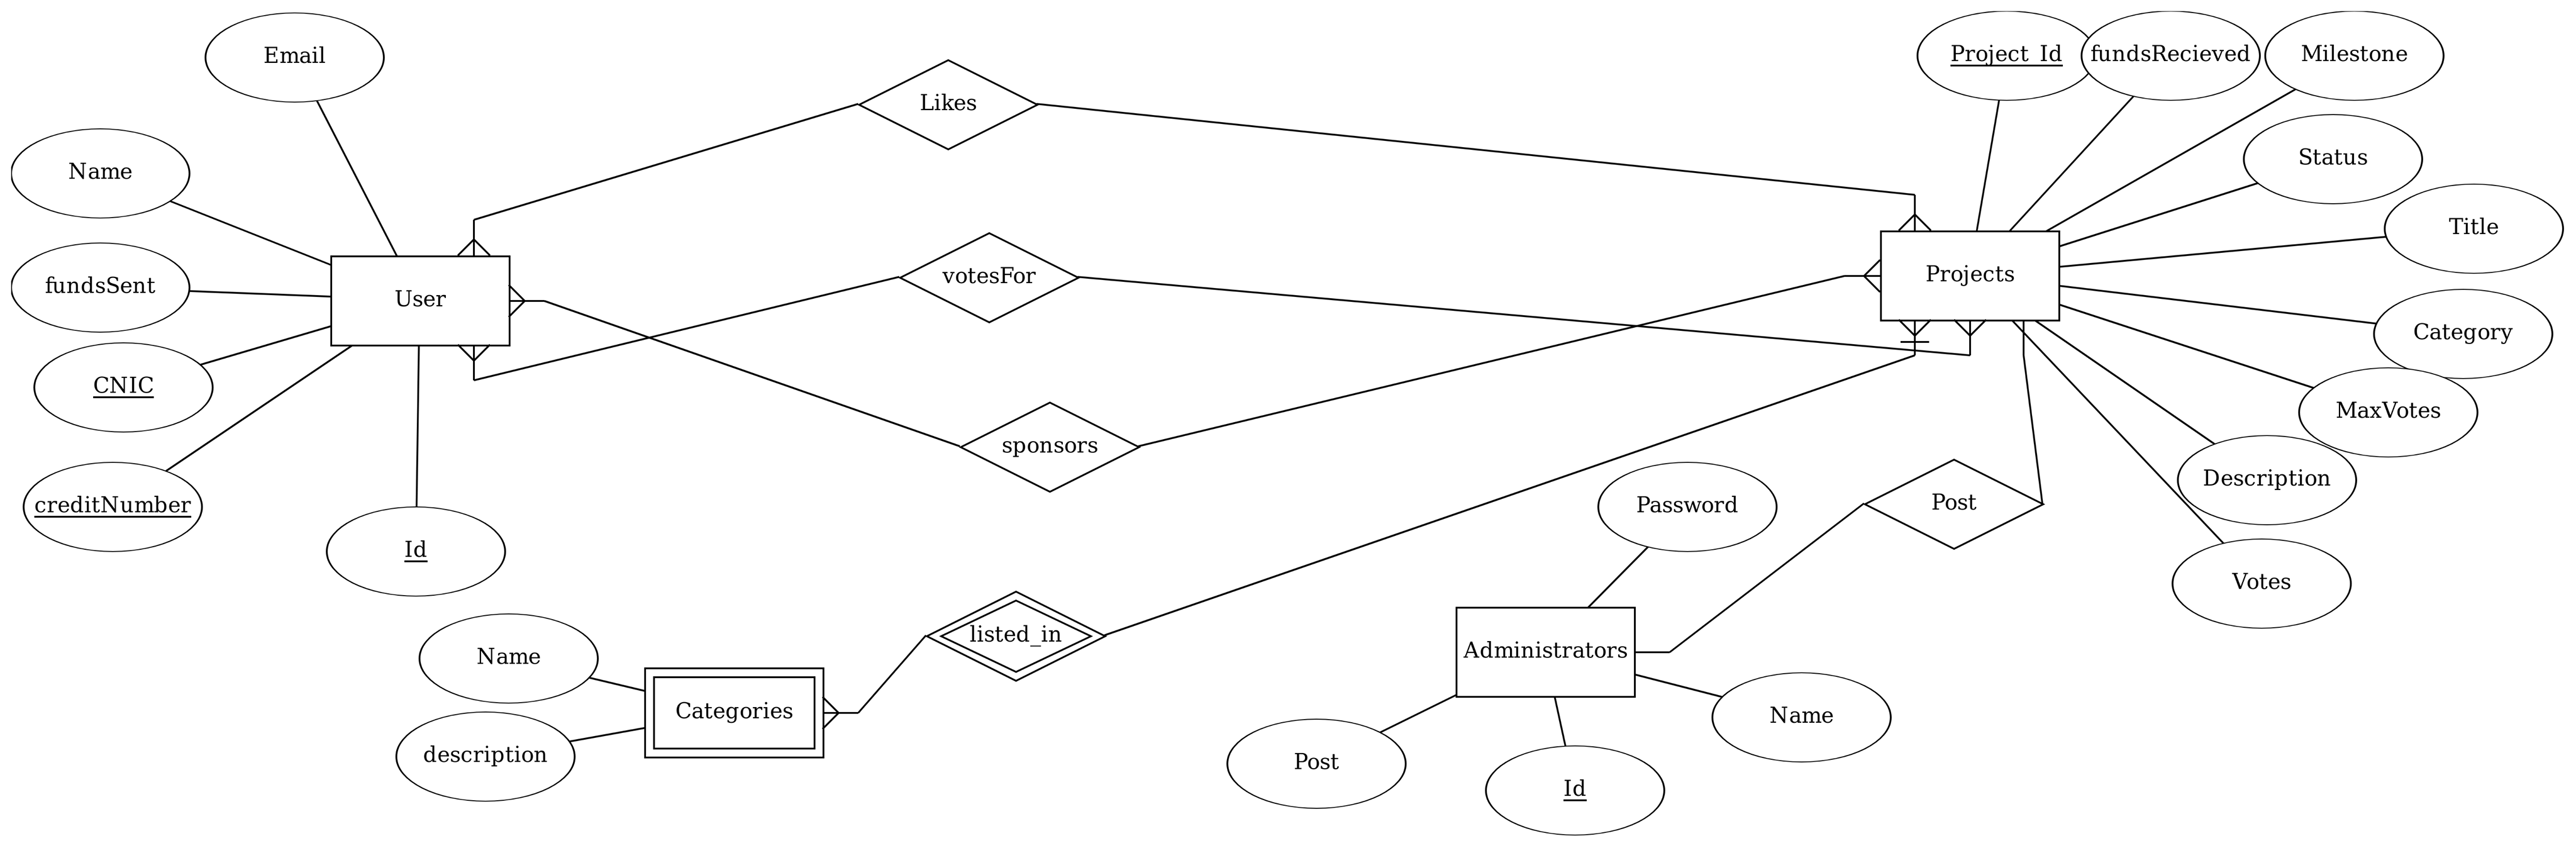
\includegraphics[width=\textwidth]{erd.png}

\subsubsection{User}
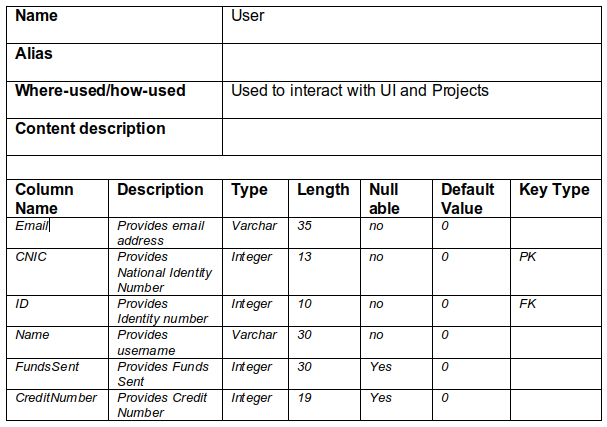
\includegraphics[width=\textwidth]{user.png}

\subsubsection{Category}
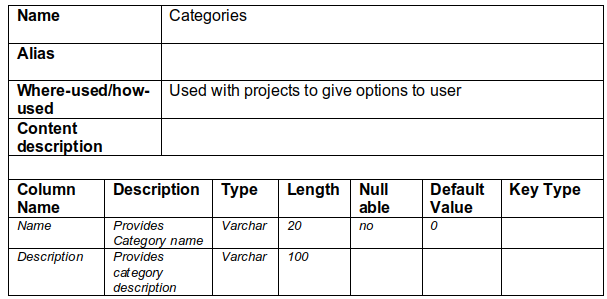
\includegraphics[width=\textwidth]{cat.png}

\subsubsection{Administrator}
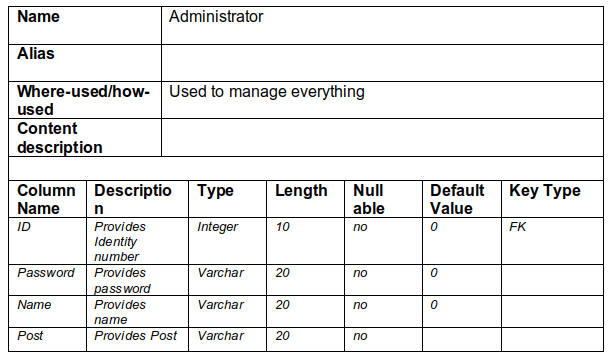
\includegraphics[width=\textwidth]{admin.png}

\subsubsection{Project}
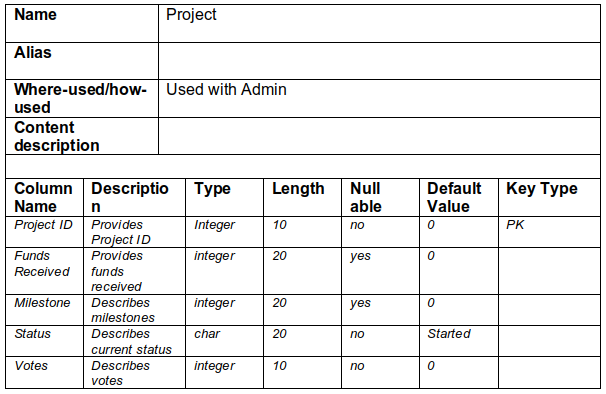
\includegraphics[width=\textwidth]{project.png}

\subsection{Application Design}
\subsubsection{Sequence Diagram}
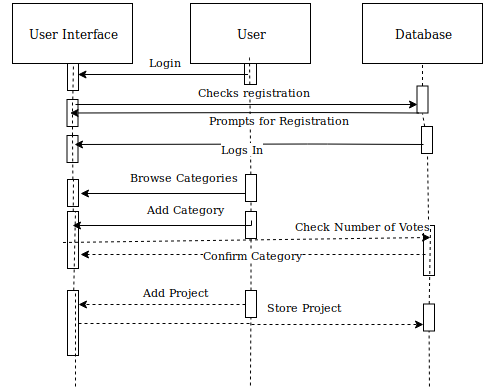
\includegraphics[width=\textwidth]{seq.png}

In this sequence Diagram we have covered three main aspects of our project:
\begin{enumerate}
    \item Login and Register: User clicks login, and enters details. The UI checks with the database if the user is registered or not and prompts if not.
    \item Add Category: In the add category function the Database checks the number of votes on the category and compares to other categories and if it fulfills or exceeds a set criteria then it is added.
    \item Add Project: The User requests a project to be added and this request is then sent to the Database which stores it.
\end{enumerate}

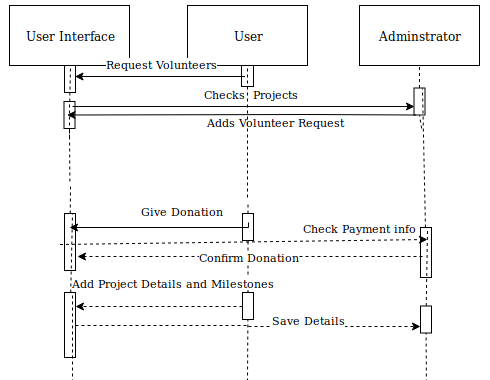
\includegraphics[width=\textwidth]{images/seq2.png}
In this sequence Diagram we have covered three main aspects of our project:
\begin{enumerate}
    \item Request for Volunteers: This is the social service and philanthropic aspect of our project. The user requests for volunteers and the project is checked by the Administrator, then the request is approved.
    \item Give Donation: This is the most integral part of our project. A user requests to donate money to a cause or project, the payment info is confirmed and then the amount is confirmed and sent back.
    \item Add project details: Here the user adds details of their project including progress, milestones achieved etc.
\end{enumerate}

\subsubsection{State Diagram}
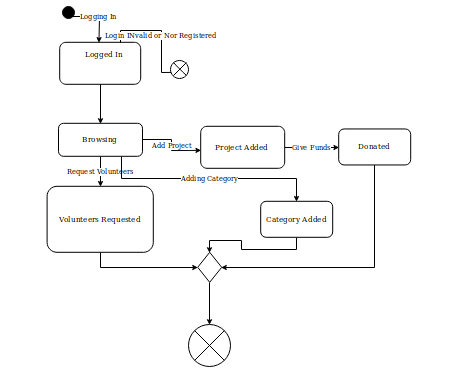
\includegraphics[width=\textwidth]{images/state.png}
Explanation:
This diagram contains all our states and starts when a user enters the logged in state. After that he enters the browsing state and can then proceed to three alternative states which are volunteers requested, category added and project added.

\section{References}
\begin{itemize}
    \item \href{http://www.agilemodeling.com/artifacts/sequenceDiagram.htm}{UML 2 Sequence Diagrams}. 
    \item \href{https://softwareengineering.stackexchange.com/questions/205061/what-is-the-general-format-of-a-software-design-specification}{What is the general format of a Software Design Specification?}
\end{itemize}

\end{document}